\section{Future work}
%\subsection{Area A}
%\frame{
%\frametitle{Proposed work: Area A}
%\begin{itemize}
%\item{\textbf{Completed: Prove robustness of DPG method for the scalar convection-diffusion problem.}}
%
%We have introduced a test norm under which the DPG method robustly bounds the $L^2$ error in the field variables $u$ and the scaled stress $\sigma$. Numerical results confirm the theoretical bounds given. 
%
%\item{\textbf{\textcolor{red}{Proposed}: Attempt analysis of the linearized Navier-Stokes system.}}
%
%We hope to analyze the linearized Navier-Stokes equations to determine an optimal extrapolation of the test norm for the scalar convection-diffusion problem to systems. 
%
%\end{itemize}
%}

%\subsection{Area B}
%
\frame{
%\frametitle{Proposed work: Area B}
%\item{\textbf{Completed: Collaborative work with Nathan Roberts on the higher order parallel adaptive DPG code Camellia.}}
%
%Numerical experiments use the higher-order adaptive codebase Camellia, built by Nathan Roberts upon the Trilinos library. %The framework for arbitrary-irregularity anisotropic refinements in both $h$ and $p$ is in place, and the code is partially parallelized.

\frametitle{Future work: anisotropic refinements and $hp$-schemes.}

The error representation function drives refinement effectively, and we hope to generalize its use to anisotropic adaptive schemes. 
\begin{figure}
\centering
\subfigure{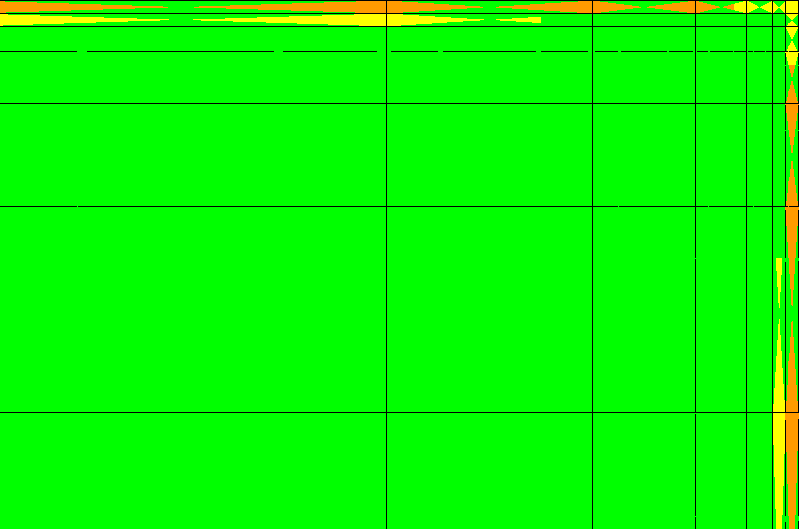
\includegraphics[scale = .175]{figs/anisotropy/b5.png}}
\subfigure{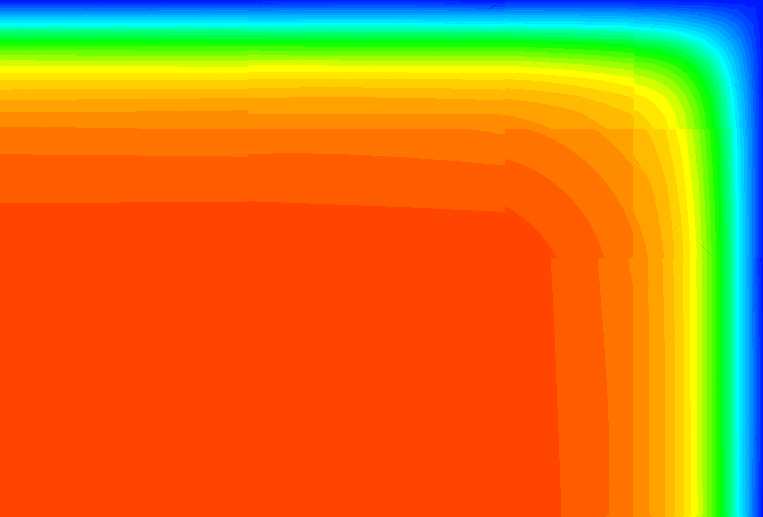
\includegraphics[scale = .18]{figs/anisotropy/v6.png}}
\caption{Anisotropic mesh for a convection-diffusion boundary layer.}
\end{figure}
}

\frame{
\frametitle{Future work: distributed iterative static condensation.}
\[
Ku = \arr{A}{B}{B^T}{D}\vecttwo{u_{\rm flux}}{u_{\rm field}} = \vecttwo{f}{g} = l
\]
where $D$ has a block-diagonal structure. The system can be reduced to yield the condensed system
\[
\left(A-B D^{-1} B^T\right)u_{\rm flux} = f - B D^{-1} g
\]
where $D^{-1}$ can be inverted block-wise. For FE stiffness matrices under the Laplace equation, the Schur complement has reduced condition number of $O(h^{-1})$ as opposed to $O(h^{-2})$.\footnote{\bibentry{schurComplement}}
}

\frame{  
\frametitle{Future work: a Nonlinear Hessian-based DPG method.}
Given a nonlinear variational problem $b(u,v) = \ell(v)$, linear in $v$ but not in $u$, beginning with the \textit{nonlinear} dual residual 
\[
J(u_h) = \frac{1}{2}\|B(u_h)-\ell\|_{V'}^2 \coloneqq\frac{1}{2} \sup_{v\in V\setminus\{0\}} \frac{| b(u_h,v)-\ell(v)|^2}{\nor{v}_V^2}.
\]
produces a Hessian-based DPG method, which solves
\[
b_u(\Delta u,v) + b''(\Delta u, \delta u, v_{R(u)}) = \ell(v) - b(u,v) = r(u,v),
\]
and aims to minimize the nonlinear dual residual instead of the linearized problem residual. 
}

\frame{
\frametitle{Future work: applications}
\begin{columns}
\begin{column}{.48\textwidth}
\begin{itemize}
\item{{Solutions for all problems over a range of Reynolds/Mach numbers.}}
\item{{Flow over a bump, Holden's ramp problem (shock-boundary layer interaction).}}
\item{{Time permitting: airfoils, regularized Euler.}}
\end{itemize}
\end{column}
\begin{column}{.5\textwidth}
\begin{figure}
\centering
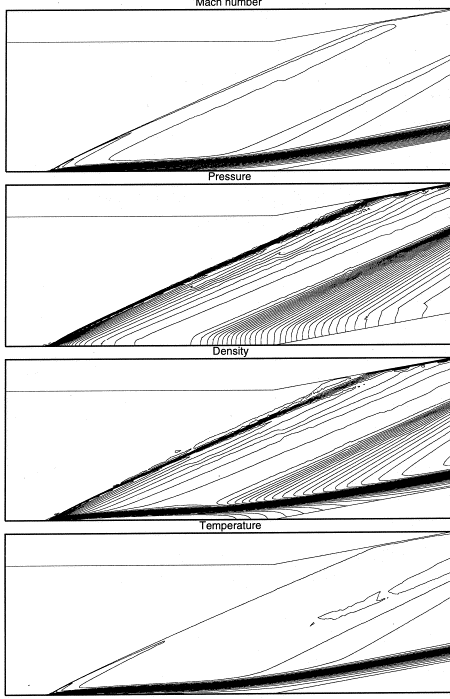
\includegraphics[scale = .275]{figs/ramp.png}
\end{figure}
\end{column}
\end{columns}
}
